\documentclass{aci}

%%%%%%%%%%%%%%%%%%%%%%%%%%%%%%%%%%%%%%%%%%
\usepackage{txfonts}
\usepackage{cite}
\usepackage{booktabs}

\usepackage{hyperref}
\hypersetup{colorlinks=true}

%%%%%%%%%%%%%%%%%%%%%%%%%%%%%%%%%%%%%%%%%%
\newcommand{\ep}{\varepsilon}
\newcommand{\eps}[1]{{#1}_{\varepsilon}}

\def\typeofarticle{Research Article} \def\currentvolume{1} \def\currentissue{1}
\def\currentyear{2021} \def\currentmonth{} \def\ppages{1--30} \def\DOI{to
appear} \def\Received{June 2022} \def\Accepted{July 2022} \def\Published{October
2022 }
%\numberwithin{equation}{section}
\DeclareMathOperator*{\essinf}{ess\,inf}

%%%%%%%%%%%%%%%%%%%%%%%%%%%%%%%%%%%%%%%%%%
\begin{document}

\title{An Ant Cuticle Texture Classification Algorithm for Ecological Anaylsis}

\author{%
  Noah Gardner\affil{1}, John Paul Hellenbrand\affil{2}, and Chih-Cheng
  Hung\affil{1}\corrauth}

% \shortauthors is used in copyright information in the end of the paper
\shortauthors{the Author(s)}

\address{%
  \addr{\affilnum{1}}{College of Computing and Software Engineering, Kennesaw
    State University, 1000 Chastain Road, Kennesaw, GA 30144, USA; email}
  \addr{\affilnum{2}}{College of Science and Mathematics, Kennesaw State
    University, 1000 Chastain Road, Kennesaw, GA 30144, USA; email}}
% corresponding author
\corraddr{chung1@kennesaw.edu}

\editor{First-name Last-name}

\begin{abstract}
  There is a large variety of ant species, and most species are diverse in terms
  of size, shape, behaviors, and especially skin (cuticle) textures. However,
  the significance of ant cuticle texture is not widely researched. This
  research employs modern machine learning methods such as texture analysis and
  classification with CNN and clustering to automatically group similar ant
  species to allow for the study of influences cuticle texture on ant ecology.

\end{abstract}

\keywords{Texture Analysis, Image Processing, Clustering, Machine Learning,
  Myrmecology, Ecology}

\maketitle
\section{Introduction}
Insects compose half of biodiversity and rank among the most dominant organisms
in terrestrial ecosystems \cite{sheikh_diverse_2017}. A key factor for the
ecological success of insects is their exoskeleton, also known as cuticle. The
cuticle protects insects from predation, provides structural support, prevents
desiccation, and serves as a canvas for advertising visual and chemical signals
\cite{gullan_insects_2009}. Research has heavily focused on the macrostructures
and internal chemical components that make the exoskeleton functional and more
recent work is being done to understand the functional aspects of external
cuticle micro sculpturing \cite{muthukrishnan_insect_2020,
  gunderson_insect_1989, watson_diversity_2017}.

Texture is an important feature in many applications, such as image processing,
pattern recognition, and computer vision. Analysis of textures can be broken
into three main categories: texture classification, texture segmentation, and
texture synthesis. The process of classifying a texture into a set of categories
and relies on three different approaches: feature-based, model-based, or
structural \cite{reed_review_1993}. In this paper, we focus on a
\textit{model-based approach} which attempt to extract parameters to reveal
common patterns and use those parameters to automatically distinguish between
different textures \cite{maillard_texture_2003}.

Although there is some work regarding grouping ants into categories of similar
cuticle, automated classification has yet to become an active area of research.
Due to the large number of different ant species, the classification of ants
into categories of similar texture is difficult to accomplish manually. Texture
analysis has shown promising results in related fields, such as plant
identification \cite{boudra_plant_2018}. With modern texture analysis methods,
the classifications of ants can be automated and the results can be used to
study the influence of cuticle texture on ant ecology.

We examine ants (\textit{Formicidae}) as they display an extreme diversity of
cuticle micro sculpturing across all subfamilies. Sculpturing ranges from
parallel longitudinal ridges to deep oval impressions to erratic protuberances.
The sculpturing has arisen convergently and independently throughout ant’s
evolutionary history, which suggests some inherent function. Cuticle sculpturing
on ants may help increase strength and rigidness, resist abrasion, increase
internal and external surface area, resist microbial growth, and rear beneficial
anti-biotic producing bacteria \cite{johnson_effect_2011,
  bruckner_relationship_2017, currie_coevolved_2006}. These specific functions may
be associated with certain sculpturing types and the purpose of classification
is to group similar textures based on proposed function.

\section{Methods}

\subsection{Sculpture Identification Protocol}

\subsection{Dataset}
In order to classify the cuticle, we used ant head images sourced from AntWeb
\cite{antweb}. In general, the ant head images are centered in the image, facing
the front, and share a similar posture. However, some images may not be
centered, show the ant head in a different orientation, or may have a
drastically different resolution from the average image. Fortunately, each can
have several scales available such that the images' scales can be roughly
similar.

\begin{table}[h]
  \centering
  \caption{Dataset Subclass Distribution}
  \label{table:classdist_all_full}
  \begin{tabular}{lll}
\toprule
Label & Samples (n) & Samples (\%) \\
\midrule
Rough Dimpled  &         173 &        0.07 \\
Rough Netted   &         503 &        0.21 \\
Rough Ridged   &         317 &        0.13 \\
Rough Tuberous &          41 &        0.02 \\
Smooth Gritty  &          16 &        0.01 \\
Smooth         &        1393 &        0.57 \\
Total          &        2443 &         1.0 \\
\bottomrule
\end{tabular}

\end{table}

\begin{table}[h]
  \centering
  \caption{Dataset Class Distribution}
  \label{table:classdist_rs_full}
  \begin{tabular}{lll}
\toprule
{} & Samples (n) & Samples (\%) \\
\midrule
Rough  &        1034 &        0.42 \\
Smooth &        1409 &        0.58 \\
Total  &        2443 &         1.0 \\
\bottomrule
\end{tabular}

\end{table}

Images were collected and classified by undergraduate students according to the
sculpturing identification protocol. Overall, there are a total of 2443 images
in the dataset. The class distribution with all considered subclasses is shown
in Table \ref{table:classdist_all_full}, and the class distribution with overall
distribution is shown in Table \ref{table:classdist_rs_full}. The relatively
small number of images in the dataset paired with the uneven class distribution
makes it difficult to perform a meaningful classification. However, the goal of
this project is to develop a classification algorithm that can be used to help
classify over 200,000 ant images. Therefore, it is desirable to use a few
representative images from each class to train the algorithm. Additionally, data
augmentation and other methods are performed to increase the number of training
images to create a more robust classification algorithm.

\section{Experimental Results}

\begin{figure}%
\centering%
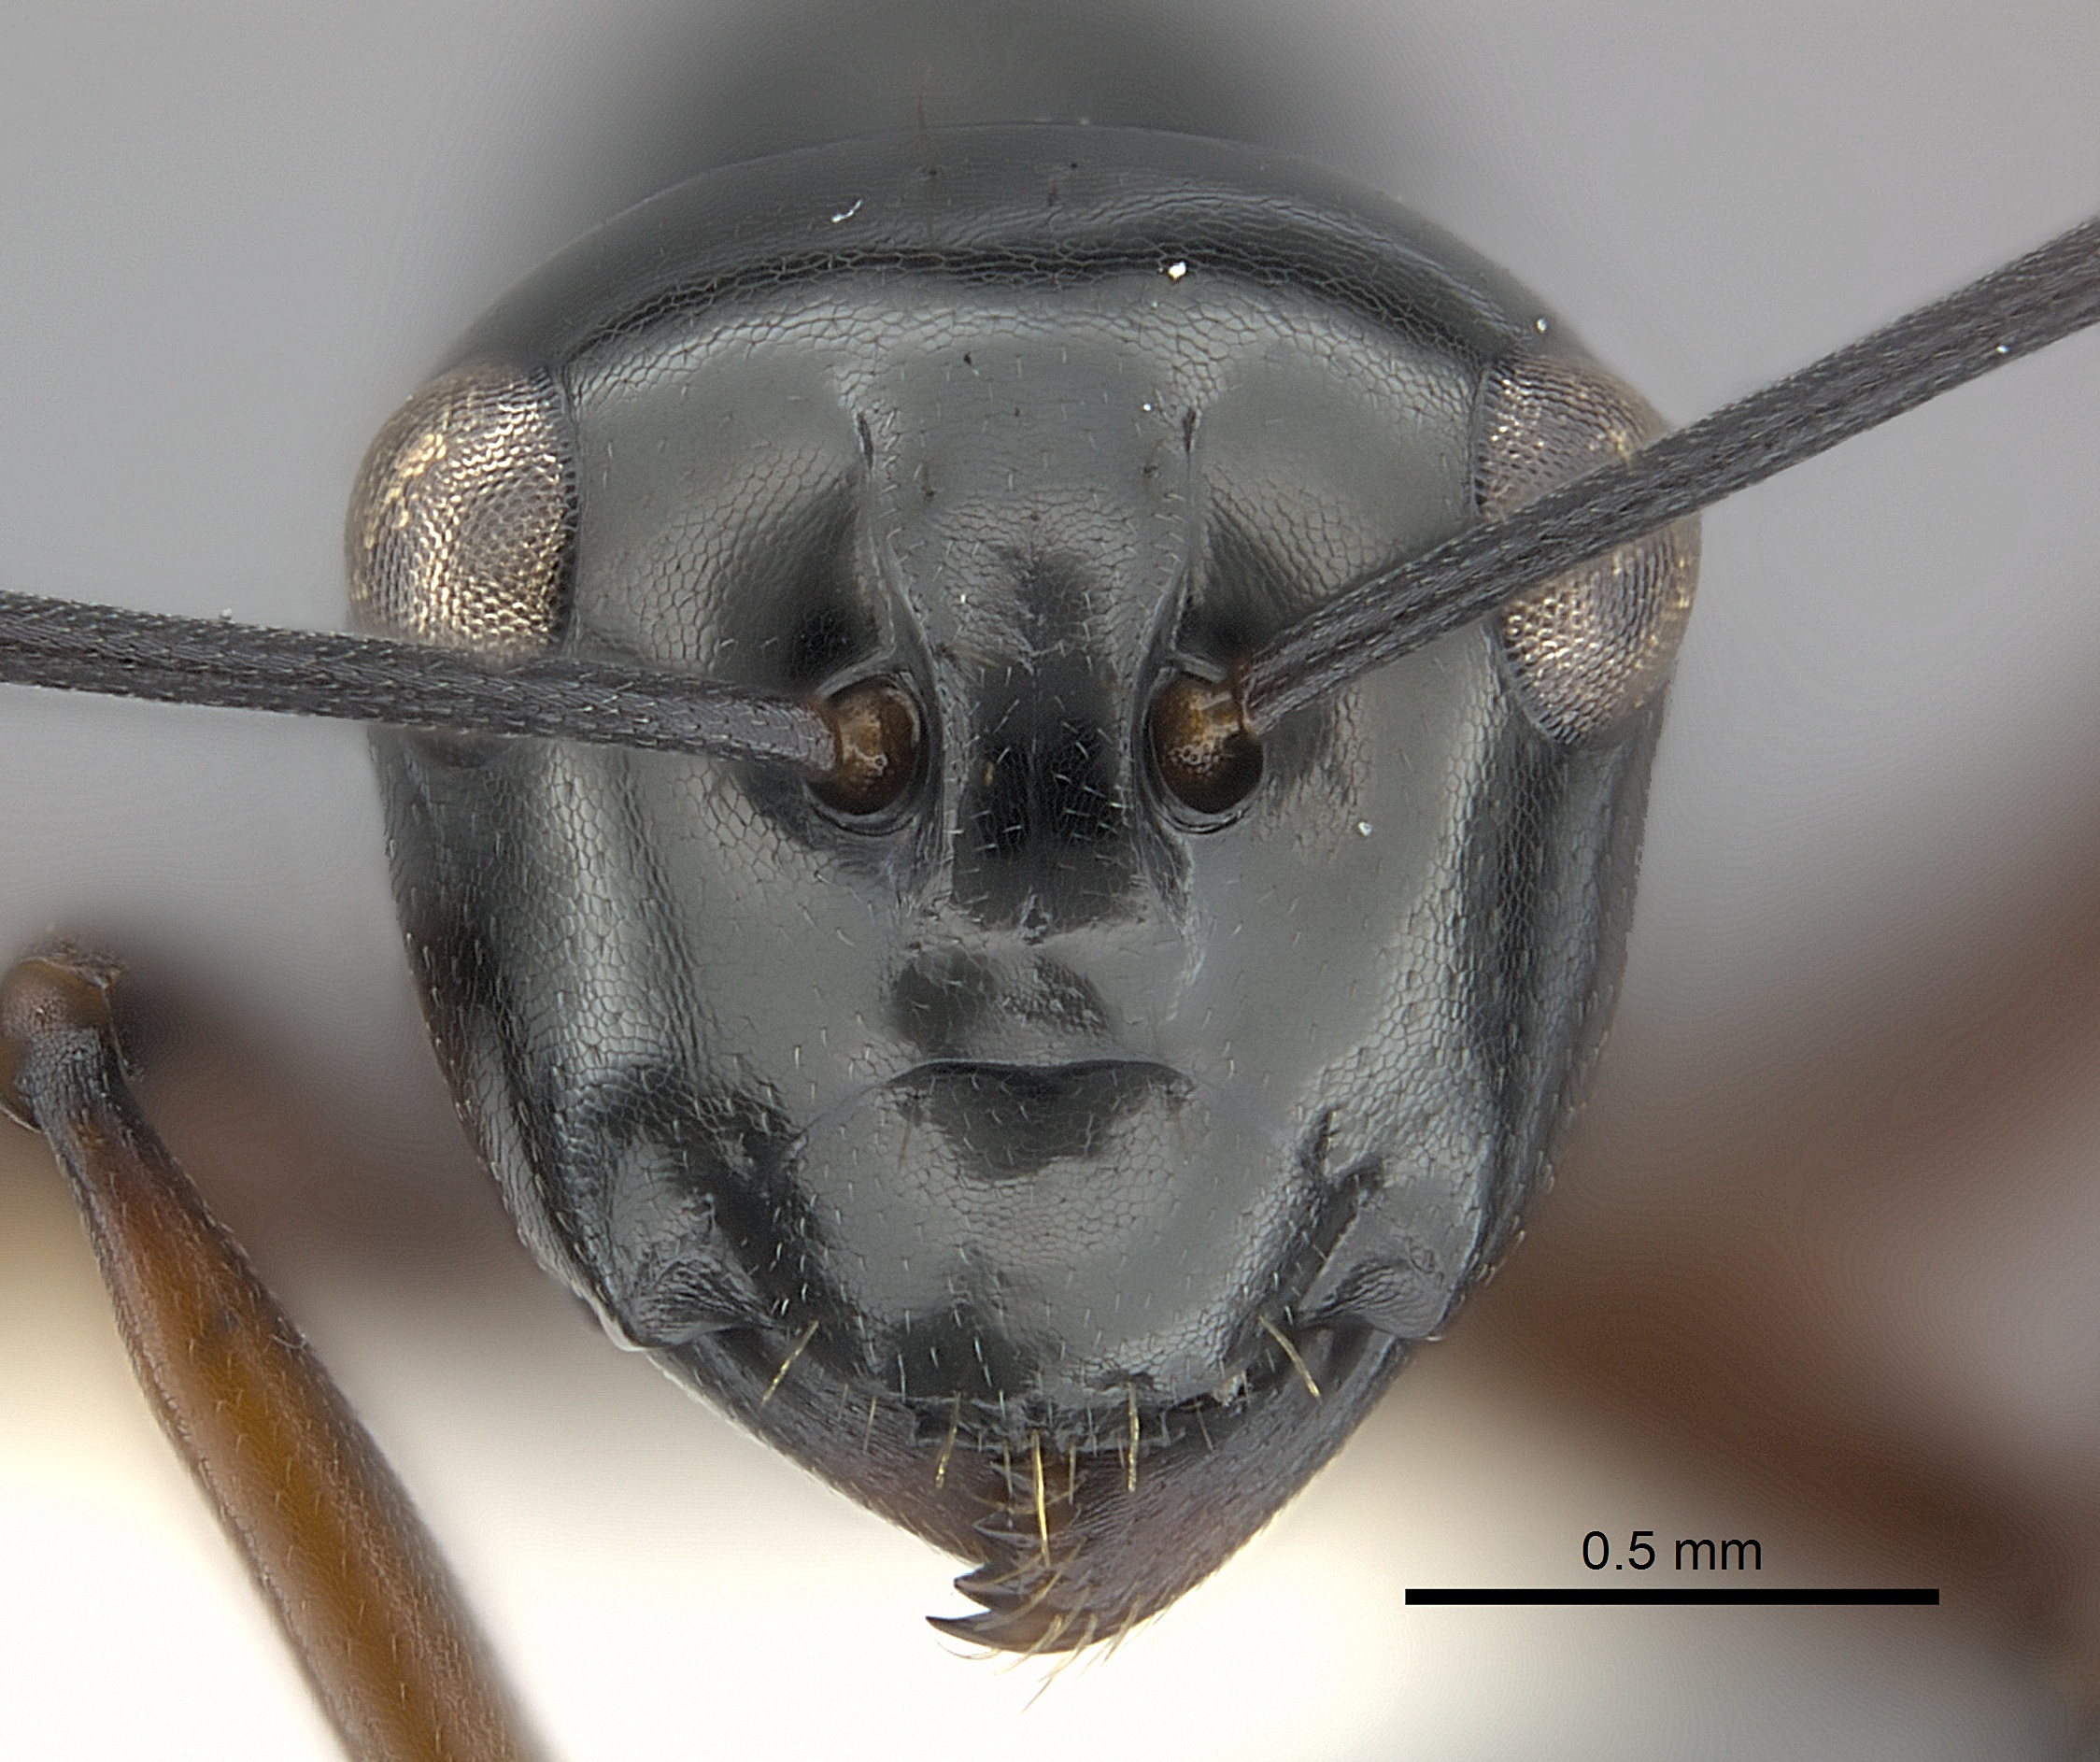
\includegraphics[width=0.2\textwidth]{assets/images/CASENT0217419.jpg}%
\caption{\href{https://www.antweb.org/bigPicture.do?name=casent0217419&shot=h&number=1}{CASENT0217419} by \href{https://www.antweb.org/artist.do?id=92}{Estella Ortega}, from \href{https://www.antweb.org}{AntWeb}}%
\end{figure}

\section*{Acknowledgments}
We would like to thank the constructive feedback provided by the reviewers.

\bibliography{paper}
\bibliographystyle{unsrt}

\end{document}
